\documentclass{standalone}
\usepackage{tikz}

\begin{document}


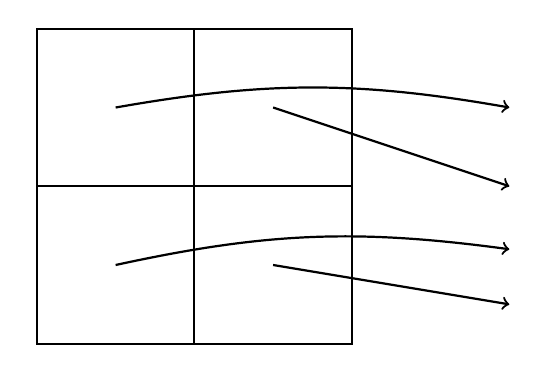
\begin{tikzpicture}

    \draw[thick] (0, 0) rectangle (4, 4);
        
        % Draw the vertical and horizontal lines
    \draw[thick] (2, 0) -- (2, 4);
    \draw[thick] (0, 2) -- (4, 2);
    
    % Draw arrows starting from the center of each block
    % Arrow from the top-left block
    \draw[thick,->,bend left=10] (1, 3) to (6, 3) node[midway, above] {};
    
    % Straight arrow from the top-right block
    \draw[thick,->] (3, 3) -- (6, 2) node[midway, above] {};
    
    % Straight arrow from the bottom-left block
    \draw[thick,->,bend left=10] (1, 1) to (6, 1.2) node[midway, above] {};
    
    % Curved arrow from the bottom-right block, bending downward
    \draw[thick,->] (3, 1) -- (6, 0.5) node[midway, above] {};

\end{tikzpicture}


\end{document}